\documentclass{article}
\usepackage{multicol}
\usepackage{graphicx,amsmath,listings,hyperref,color,appendix,geometry}
\usepackage[english]{babel}
\usepackage{graphicx}
\usepackage{float}
\usepackage{mathtools}



\begin{document} 
\begin{figure}[!bh]
 	\begin{center}
 	 
 		\huge \title{Impacts of the HTTP/2 protocol for large scale web environments}
		\author{Martin Leucht, James Gratchoff \\
		Master SNE \\ University of Amsterdam} 
		
\includegraphics{images/uva.jpeg}
	\maketitle 
		\label{sec:uva}
	\end{center}
\end{figure}
\pagenumbering{gobble}
\setlength{\columnsep}{2cm}
\def\columnseprulecolor{\color{blue}}
 
\newpage
\tableofcontents

\pagenumbering{arabic}
\newpage
\section{Introduction}
\label{chap:intro}
The well known version 1.1 of the HTTP protocol is used since 1999 for browsing the web. It is a protocol that has been reviewed many time to the point that the IETF has split the original RFC (2616\cite{RFC2616}) into six different ones (7230-7235\cite{RFC723x}) describing the whole protocol in details. After more than 15 years of use it was time for a change. All the tricks not to slow the HTTP/1.1 protocol have to be forgotten as on February the 18th 2015, the specification \cite{http2} for the new HTTP protocol HTTP/2 (and HPACK\cite{hpack}), has been formally approved by the IESG and is on the way to become an RFC standard.   \\
The main focus during the development period of the successor of HTTP/1.1 was to improve the performance, and thus provide a better user experience. The performance improvement is based on how the packets are sent over the wire within a HTTP/2 session. HTTP/2 data is sent in binary format and instead of creating a single TCP session per element retrieved, HTTP/2 create TCP streams that are multiplexed and that can be prioritized. The goal of this technique is to reduce the high number of TCP sessions created every time a user access a web page. Concerning security, HTTP/2 will not make the use of TLS mandatory. However, leading browsers firms, Mozilla Firefox and Google Chrome have already mentioned that HTTP/2 will only be implemented over TLS. Thus ensuring that the data will be encrypted between two end parties. HTTP/2 introduces several other new features that will be presented in this paper. \\
There are already web client and server implementations\cite{http2-imp} that support the final HTTP/2 specification. This research is intending to show what are the impacts of implementing HTTP/2 with TLS compared to HTTPS in a large environment. The implemented server will be tested with a high number of virtual clients located at different places around the world to outline the impact of the round trip time (RTT) on both version of the protocol and to see which performs the best. The research will draw conclusions on what impacts does the new protocol can have on large web service providers infrastructure.
\newpage
\section{Research Questions}
\label{chap:rq}
To conduct the research the following research questions have been formulated: \\
\\
How do the new features of the  HTTP/2 protocol improve the performance for frequently visited webpages/webserver? 
\\
\\
That question can be narrowed down to some sub questions:

\begin{itemize}
\item What are possible drawbacks that can occur for large web service providers when switching from HTTP/1.1 to HTTP/2 ?
\item What is the predictable impact that could be related to changes in the infrastructure of Web service providers?
\item What is the difference in bandwidth utilization between HTTP/1.1 and HTTP/2 considering the size ratio of header and data for multiple concurrent sessions on a server?
\item How much can HTTP/2 decrease the amount of data when considering header compression and using multiple streams within one TCP Session compared to HTTP/1.1 on a server ?
\item What is the impact regarding the response time experienced by a client when the number of concurrent requests / clients increases seen from three different geographical locations?
\item What is the impact to the load and CPU utilization to the server when conducting the benchmark tests?
\end{itemize}
\section{Scope}
\label{scope}
The scope of this research is to conduct benchmarks of the HTTP/1.1 and HTTP/2 protocol, using different static and dynamic parameters and compare them among each other. Static parameters are the distance between client/server (RTT) and the page size, whereas dynamic parameters are the number of requests and the number of concurrent clients. Therefore we will implement three different HTML pages with different sizes and benchmark them from three different geographical locations. The tests will be implemented using the secured version of the protocols with TLS enabled. We do not focus on implementing the new features of the HTTP/2 protocol like server push capabilities.  


\newpage
\section{Literature review}
\label{relwork}
The creation of the HTTP/2 protocol have been discussed for many years. This section discusses the drawbacks of the previous version and presents the reasons why to move to a new protocol. The features that will improve the performance of the HTTP/2 protocol are also introduced. And finally the related work section will present the benchmarks that have been done for the SPDY and HTTP/2 protocol.

\subsection{HTTP/1.1 drawbacks}
Specified in multiple RFCs(7230-7235), HTTP/1.1 is a standard protocol for web-browsing that is now used for more than 15 years. This protocol has been reviewed a number of times and contains a high number of options. It uses a client-server model where the clients is most of the time a browser that is getting data from a server located in a different location. HTTP is the essence of the web and most of the users are using this protocol on a daily basis. 
Since the early beginning of the protocol, users complained about the time that takes a page to load. One big reason of this problem was not due to the protocol but to the speed and the reliability of the Internet. However the web has changed and more and more users have a high speed and reliable connection to the Internet. This and the growth of clients on the web has led to the increase of web pages size and the number of elements on a web page. HTTP was not designed for this use as indeed it is inadequately using the TCP protocol by retrieving one element from a web page using one TCP connection. It is thus not taking full advantage of the high performance TCP protocol as indeed the current use of TCP in HTTP/1.1 protocol can introduce problems that are leading to a slower loading time. These problems are for example the head of line blocking or the repetition of headers between multiple TCP sessions. The loading time is also highly dependent on the Round Trip Time (RTT) and some efforts have been done on improving this aspects over the years by adding geographical redundancy however the problem is still present for low cost organisation that are only able to develop server in a single location. 
This latency directly affect the clients and can be critical for your website (e.g. users leaving the page as it takes too long to load). So over the years, web developers have tried to reduce this critical factor that is latency. In order to do so the developers have been tried to adapt themselves to the protocol with workarounds that reduce the number of TCP connection. The most known workarounds are:
\begin{itemize}
\item Spriting: The fact to create an image containing many pictures destined to be present on the website and let the browsers display (via CSS or Javascript) the picture wanted by cropping/cutting out a single image.
\item Sharding: In order to overcome the problem of increasing TCP connections per domain, developers started to create several domains, holding different part of the website. This decreases the page loading time by reducing the number of connection per domain. Thus leading to a better performance of the HTTP/1.1 protocol. This method can also be used to allow more TCP sessions as each domains are bounded to a certain number.
\item Concatenation: In order to reduce the number of TCP connections, developers started to concatenate files (e.g. javascript) into one big files. 
\item Inlining: By embedding the data straight in the CSS in base64 format it avoids to send picture and thus creating new TCP connections. 
\end{itemize}
All these workarounds were needed as the page loading time and the number of requests were increasing so much that the web was slowing down even though more and more people had access to a reliable connection. After 15 years, it was time for a change. That is why the IETF created a working group named HTTPbis that started working on a new protocol. Beforehand Google started working on a new protocol, called SPDY, that was aiming to encounters the problems from the HTTP/1.1 protocol. The HTTPbis group started working from a working concept of protocol in the name of SPDY/3 (draft). And this was the start of HTTP/2.

\subsection{HTTP/2 improvements}
This section is subdivided into several ones describing the major improvements made from its predecessor HTTP/1.1 and emphasis on the reasons to move to the new HTTP/2 protocol for large scale environments. 

\subsubsection{Binary format}
HTTP/1.1 is based on a text/ascii format which is an advantage for humans to read and thus to debug the protocol. It is described by Raymond as "easy for human beings to read, write, and edit without specialized tools"(http://www.catb.org/esr/writings/taoup/html/ch05s01.html). However for computers such as clients and server, ascii is not their mother tongue. Indeed computers are using binary as a format for exchange. HTTP/2 is using this format.
"HTTP/2 also enables more efficient processing of messages through use of binary message framing."(https://datatracker.ietf.org/doc/draft-ietf-httpbis-http2/?include\_text=1) Binary is know to be much more efficient for binary structures. It is indeed hard to define the start and the end of a field in text based protocols. However with binary format it is much more natural. Binary will then improve the structure of the protocol and thus the efficiency of the protocol. In order to overcome the difficulty of debugging the binary protocol, tools such as curl have added support for HTTP/2 and Wireshark have created extensions to decode the network streams.

\subsubsection{Multiplexing and priority}
The use of streams is a major enhancement of the HTTP/2 protocol. A stream is described in the specification as "an independent, bi-directional sequence of frames exchanged between the client and server within an HTTP/2 connection." The stream identifier, present in the header format as an integer, will associate each frame belonging to the same stream. One HTTP/2 connection can contain several concurrently open stream, that can each be closed by the client or the server. Streams are multiplexed which can mean that they do not arrive at the same order as they have been sent. It is the role of the client to put this streams back together in a correct order to process the data. 
Each stream has a priority that can be set by the client in the HEADERS frame that opens the stream. This priority can be changed to re-prioritize a specific stream. This can permit to avoid the head of the line blocking and allow an endpoint to express how it would prefer to retrieve data when managing multiple concurrent streams.  A stream can also be dependent on other streams by setting the stream dependency parameter.

\subsubsection{Header compression}
One of the problem of HTTP/1.1 described earlier is that more and more elements are retrieved per web page. If too elements are close in type and location the headers will be very similar and "thus the redundant header fields in these requests unnecessarily consume bandwidth, measurably increasing latency. " (http://http2.github.io/http2-spec/compression.html) That is why header compression is a good solution to this problem. However HTTPS and the SPDY compression mechanism have been vulnerable to the BREACH and CRIME attacks. That is why the HTTPbis group has created HPACK (Header Compression), that is the specification that comes with HTTP/2. HPACK is described as "simple and inflexible." It eliminates redundant header fields and prevent security issues.

\subsubsection{Flow control}
The flow control is implemented in HTTP/2 by assigning an integer value to a window that will define how many octets of data the sender (server) is able to transmit. In that way the server is taking in consideration the buffering capacity of the receiver. This has enormous advantages as receivers on the web can be of different nature (e.g.Smartphones, laptop) with different connection. Flow control control can either operate on the entire connection or on each individual stream. The default value is 65535 octets. In order to reassign this value the receiver (client) can send a SETTINGS frame with his flow control integer value.

\subsubsection{Server push}
HTTP/2 allows the server to send extra information with a requested information required by a client. This functionality permits to increased the overall loading time by anticipating what the client will need before it asks for it. In that way the client will already possess the information when asking for it. This is called the server push mechanism. This mechanism is not required but can improve the user experience. The client must allow the server to do so. This allow the client to stay in control and indeed the client is able to terminate that pushed stream by sending a RST\_STREAM.

\subsection{Related work}
The new HTTP2 protocol has been based on the SPDY protocol developed mainly by Google. As shown by Google \cite{google2x}, the SPDY protocol meets its expectations by reducing the loading time of web pages by 55\%. Other people have tried to look into the protocol and one of the most interesting analysis has been done by Servy\cite{servy}. Servy evaluated the performance of the web servers implementing the SPDY protocol comparing it to HTTP/1.1 and HTTPS. The load testing tool used for this benchmark was the NeoLoad 4.1.2. His results showed that the implementation of SPDY increases by a factor of 6 the number concurrent of users possible before errors start showing up in comparison to HTTP and HTTPS. 
A contradictory study showing some boundaries of implementing SPDY has been done by Podjarny\cite{podiatry}. He shows that most of the websites use different domains and as SPDY works on a per-domain basis it does not necessarily help it to be faster. Finally, Wang et al.\cite{wang} have investigated the performance of SPDY for the improvements of the protocol compared to HTTP/1.1. This study highlights that SPDY is much faster since its benefits from the single TCP connection mechanism. However, they also mention that SPDY degrades under high packet loss compared to HTTP. 
Concerning the new standard HTTP/2 a few benchmarks have been performed by the creators of different client/server platforms. They reach the same conclusion for SPDY. \\
However, studies on comparisons between HTTP/2 (draft-ietf-httpbis-http2-14 \cite{h2c-14} ) and HTTP/1.1 with regards to concurrent clients and increasing amount of requests in different geographical locations and different page sizes or amount of elements a web page contains, have not been conducted yet.

\subsection{Conclusion}
To conclude, this section presented the reasons that have lead to the design of a new version of the HTTP protocol. The TCP protocol have been implemented in the early days of the HTTP protocol however due to the evolution of the web the protocol started lacking and the principal reason was that the use of the TCP protocol was not suiting the web usage any more. HTTP/2 address these issues by exploiting in a better way the TCP protocol. It also creates new features that will redesign the way to implement large infrastructure such as flow control, stream priority or server push. The new performance of the protocol have been tested by the designers of the implementation of the protocol but not by other parties. That is why this research has been conducted.
\newpage
\section{Approach and Methods}
\label{sec:approach_and_methods}



\subsection{Measurement}
\subsubsection{Measurement Parameter}
\label{subsec:measurements}
To perform various measurements that reflect realistic scenarios a large web content provider will encounter, a topology consisting of several components was composed. As HTTP client machines, Amazon AWS microinstance VMs \cite{amazon} located at different geographical locations (Europe, North America and Asia) are used. Different geographical locations used on client side, ensure to perform measurements seen from different magnitudes of Round Trip Times towards the destination web server located in Amsterdam. On server side two TLS enabled webserver instances are running on one physical machnine in order to conduct measurements for both protocols - HTTP/1.1 and HTTP/2. Three reference HTML pages of different sizes and different numbers of statically linked resources have been created to be compared. These pages reflect the sizes that can be encountered in most common websites and has been derived from top 100 websites statistics \cite{httparchive}. The appropriate web page sizes including the number of resources are listed in Table \ref{table:pages}.

\begin{table}[h]
	\centering
\begin{tabular}{ | c | c | c | }

\hline
\textbf{Web Page} & \textbf{Size (kB)} & \textbf{Number of links}\\ \hline \hline
small.html &  20 & 2 \\ \hline
medium.html &  600 & 7\\ \hline 
large.html &  1600 & 54 \\
\hline
\end{tabular}
\caption{different Web Pages}
\label{table:pages}
\end{table}

So far, we have defined different static parameters that will be applied while performing the measurement. These parameters include different Round Trip Times (RTTs) and different webpage sizes.  
To simulate varying and realistic load scenarios on the server, the number of clients and thereby the number of requests towards the webservers is incremented during each test starting from one client upto maximal 750 clients in parallel.
\\  
\subsubsection{Measurement Tools}
It is essential to choose and implement the right tool and method to measure the response/request times characteristics of the HTTP/1.1 and HTTP/2 protocol and to be able to compare them with each other. Thus, the bechmarking tool was chosen carefully and with respect to retrieve accurate measurement data that can be used to compare both HTTP versions with each other. 
H2load \cite{h2load} was elected as the best candidate for that purpose. It has been developed to run benchmarking tests against HTTP/2 enabled webservers. 
It can also be used to conduct measurements against HTTP/1.1 enabled web servers if, like in that case, a HTTP/2 - HTTP/1.1 reverse proxy is used that is capable to translate HTTP/2 requests into HTTP/1.1 requests on server side. 
It is possible to start h2load with a file option, that includes a list of URIs that each measurement will request in parallel. H2load returns after each measurement round accurate and valuable data, like the retrieved  amount of header and body data in bytes per request. Furthermore it returns the minimum, maximum and mean round trip time for each web page request and the actual performance in requests/second. 
\\
\subsubsection{Measurement Methods}
In order to collect statistical analysable data, all measurements are performed with twenty repetitions. A wrapper script was created that performs the measurements using h2load, does mean calculations on the data and writes them into a file. The data is later processed for visualizing round trip times and other measurements. The wrapper script can be found at the end of that report as part of the appendices. 
\\
It is important to notice that the main difference between HTTP/1.1 and HTTP/2 sessions is based on the number of created TCP sessions on server side. A HTTP/1.1 client (e.g. web browser) opens for each HTML link that is present in a HTML webpage a separate TCP session to the webserver. In contrast to HTTP/1.1, the new HTTP/2 protocol opens one single TCP session towards the server and multiplexes all requested data over multiple streams within a single TCP session. Thus, the maximum number of concurrent streams for each HTTP/2 session is set equal to the amount of requested URIs in all measurements. Figure \ref{fig:httpwatch} shows HTTP/1.1 GET requests in order to get the entire set of resources the reference webpage (large.html) includes.


\begin{figure}[H]
	\centering
	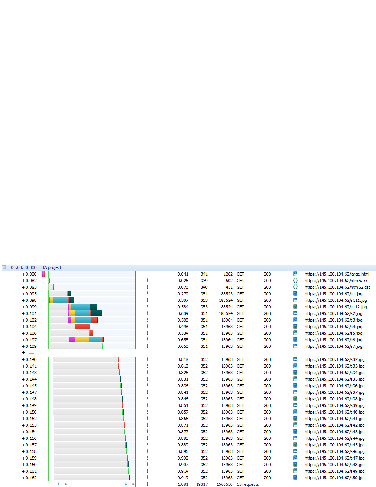
\includegraphics[scale=2,trim=0.0cm .0cm .0cm 4.5cm,clip]{images/http.pdf}
	\caption{HTTP/1.1 GET requests for large.html}
	\label{fig:httpwatch}
\end{figure}

HTTP/2 handles all GET requests in a single TCP connection by using multiple streams \textit{s}, thus the expected number of TCP connections \textit{t} will be equal to the number of concurrent simulated clients \textit{n}. For HTTP/1.1  we expect the number of TCP connection \textit{t} as a function of the product of concurrent clients \textit{n} by the requested number of HTML links \textit{l}. Thus we can describe the number of TCP sessions for HTTP/1.1 as \begin{equation}
t=f(n)=n*l \qquad \text{and} \qquad l \geq 1\end{equation} and for HTTP/2 as \begin{equation} t=f(n)=n \qquad \text{and} \qquad s=l; l\geq 1; s \in n \end{equation}

That results in Table \ref{table:tcpconnects} which shows the expected numbers of TCP connections towards the webserver during some stages in the measurements with an assumed number of \textit{l=55} HTML links per page request.

\begin{table}[h]
	\centering
\begin{tabular}{ | c | c | c | }

\hline
\textbf{clients/requests \textit{n}} &\textbf{\textit{t} (HTTP/2)} &\textbf{\textit{t} (HTTP/1.1)}\\ \hline \hline
1 & 1 & 55 \\ \hline
10 & 10 & 550\\ \hline
50 & 50 & 2750\\ \hline
150 & 150 & 8250\\ \hline
300 & 300 & 16500 \\ \hline
500 & 500 & 27500\\ \hline 
750 & 750 & 41250\\
\hline
\end{tabular}
\caption{Number of TCP connections HTTP/1.1 and HTTP/2}
\label{table:tcpconnects}
\end{table} 
%%\subsection{Overview}
\label{subsec:topology}
For our measurements we have setup a benchmark topology consisting of Amazon AWS microinstance \cite{amazon} clients located at different geographical locations (Europe, North America and Asia). That ensures to perform measurements seen from clients with  different Round Trip Times to the destination server located in Amsterdam. On the server side, in Amsterdam, different webserver implementations are used in order to conduct measurements for both protocols - HTTP/1.1 and HTTP/2. 
\\
Three reference HTML pages of different sizes and different numbers of statically linked resources have been created to be compared. These pages reflect the sizes that can be encountered in most common websites and has been derived from top 100 websites statistics \cite{httparchive}. The page sizes including all resources, are listed in Table \ref{table:pages}.

\begin{table}[h]
	\centering
\begin{tabular}{ | c | c | c | }

\hline
Web Page & Size (kB) & Number of statically linked resources\\ \hline \hline
small.html &  20 & 2 \\ \hline
medium.html &  600 & 7\\ \hline 
large.html &  1600 & 54 \\
\hline
\end{tabular}
\caption{different Web Pages}
\label{table:pages}
\end{table}

So far, we have defined different static parameters that will be applied while performing the measurement. These parameters include different Round Trip Times (RTTs) and different webpage sizes. To simulate varying and realistic load scenarios on the server, the number of clients and thereby the number of requests towards our webservers is incremented during each test from one client upto maximal 750 clients in parallel. Figure \ref{fig:httpwatch} shows all required HTTP/1.1 GET transactions in order to fetch the entire set of resources included in the large variant of the reference webpage (large.html).

\begin{figure}[H]
	\centering
	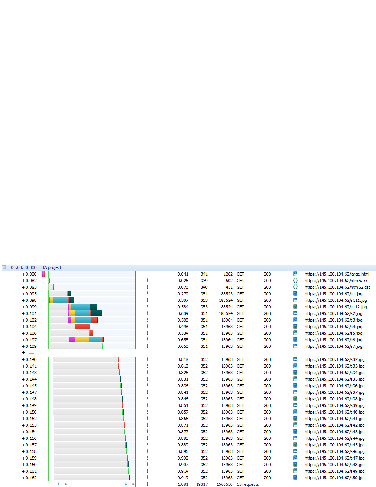
\includegraphics[scale=2]{images/http.pdf}
	\caption{Page Requests for large.html}
	\label{fig:httpwatch}
\end{figure}
  

It is essential to choose and implement the right tool to measure the response/request characteristics of the HTTP/1.1 and HTTP/2 protocol and to be able to compare them with each other. Thus, the bechmarking tool was chosen carefully and with respect to retrieve measurement data that can be used to compare both HTTP versions with each other. 
\\
H2load \cite{h2load} was the best candidate for that purpose. It has been developed to run test against HTTP/2 enabled webservers. i
It can also be used to conduct measurements against HTTP/1.1 enabled servers if, like in that case, a HTTP/2 - HTTP/1.1 reverse proxy is used taht is capable to translate HTTP/2 requests into HTTP/1.1 requests.    

\subsection{HTTP Server and Clients}
\label{subsec:server_client}
HTTP clients that conduct measurements from long distances are deployed using Amazon t2.micro instances. T2 instances provide a baseline level of CPU performance that is comparable to 2 vCPUs with the ability to burst above the baseline level \cite{amazon-ts}. For local tests within the OS3 network, XEN VM are used. Each client got at least 2 vCPUs and 2 Gigabyte RAM assigned. The clients are located in different geographical areas, resulting in different RTT times between clients and server. On each client h2load was compiled and the wrapper script uploaded. Table \ref{table:locations} shows all clients and their corresponding average round trip times to the server.

\begin{table}[h]
	\centering
\begin{tabular}{ | c | c | }

\hline
\textbf{Location} & \textbf{RTT in ms}\\ \hline \hline
Tokyo/Japan &  280\\ \hline
North Carolina/US &  150\\ \hline 
Frankfurt am Main/Germany &  7\\ \hline
Amsterdam/Netherlands &  0.3\\

\hline
\end{tabular}
\caption{RTT (in ms) per location}
\label{table:locations}
\end{table}

The server that provides access for the HTTP clients is not virtualized. It has 8 Intel Xeon CPUs (1,87GHz) and 8GB RAM installed. The webserver has a public IPv4 address and is connected to the public internet via a 1 Gbit Ethernet interface. As HTTP/2 server nghttpd \cite{nghttp} is used which listens on TCP port 8881. For HTTP/1.1 requests Apache2 \cite{apache} in combination with nghttpx \cite{nghttpx} is used. Nghttpx is a reverse proxy and accepts HTTP/2, SPDY and HTTP/1.1 over SSL/TLS on TCP port 8443 via its frontend. The protocol to the backend is HTTP/1.1. The usage of an reverse proxy enables us to use our measurement tools without modification, although native HTTP/1.1 requests instead of using a reverse proxy would probably result in more accurate measurements. Since our time was very limited, we decided us to go for the reverse proxy option.


\newpage
\section{Results analysis}
\label{sec:results}
In that section the measurement results are presented and analysed. First the HTTP header sizes for HTTP/2 and HTTP/1.1 are compared against each other. Second, the results of the RTT measurements and the actual performed rate of requests per second with a growing number of concurrent clients are presented and discussed. Finally an overview of the server utilization during the measurements is given for network bandwidth, CPU utilization and TCP sockets.  
\subsection{HTTP Header Size}
\label{subsec:header_size}

HTTP/2 uses HPACK \cite{hpack} as a header compression mechanism in order to decrease the amount of data for repetitive HTTP header information. Figure \ref{fig:headersize} shows the difference between HTTP/2 and HTTP/1.1 regarding the amount of header depending on the amount of clients.

\begin{figure}[H]
	\centering
	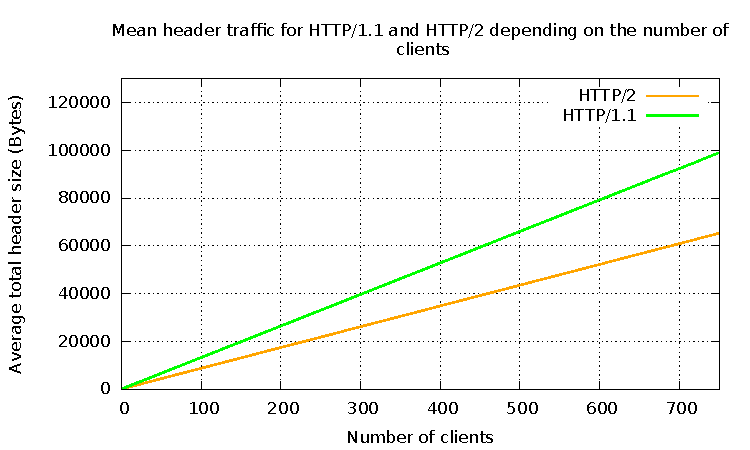
\includegraphics[scale=1,trim=0.0cm .0cm .0cm .0cm,clip]{images/headertraffic.pdf}
	\caption{header traffic in bytes for HTTP1.1 and HTTP/2}
	\label{fig:headersize}
\end{figure}

The result is a linear graph for both versions with a higher rate of growth for HTTP/1.1. It turns out that in our measurement setup the amount of traffic produced to transmit HTTP headers is approximately 30\% lower for HTTP/2 compared to HTTP/1.1. 

\subsection{HTTP Round Trip Times and Request Rates}
\label{subsec:rtt}

In that section the RTT time seen from different locations with a growing number of clients is presented. Furthermore the performance in requests per second is shown. The test are shown by location ordered by decreasing distance to the server

\subsubsection{Tokyo/Asia}

The measurements in asia are performed with the highest RTT of 280 ms. The graph in Figure \ref{fig:latency-asia}  represents the data for 4 measurements by using for each HTTP version two different pages (20kB, 1600kB). The number of clients is incremented by one  from 1 to 750, while performing the measurements.

\begin{figure}[H]
	\centering
	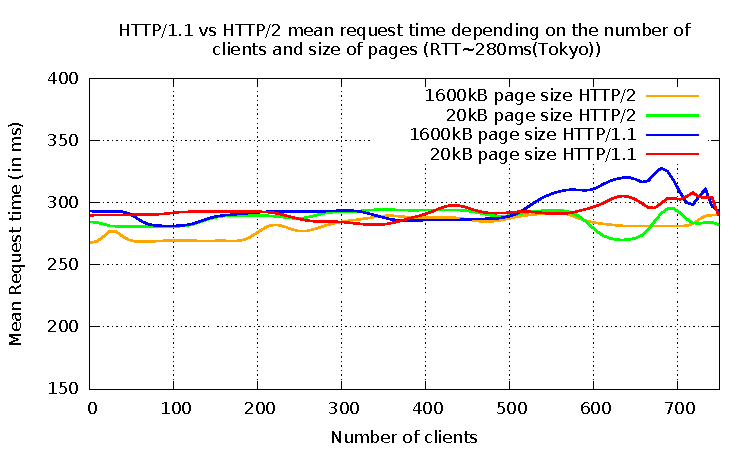
\includegraphics[scale=1,trim=0.0cm .0cm .0cm .0cm,clip]{images/latency-asia.pdf}
	\caption{Mean RTT measurements for Tokyo/Asia}
	\label{fig:latency-asia}
\end{figure}

A significant difference between both HTTP versions cannot be identified, although HTTP/2 is a few milliseconds faster during the measurements. The graph shows nearly a constant response time regardless if the number of clients increases. That can be explained by considering the rate of requests per seconds seen from the client in Tokyo. As more clients are added as more requests are beeing executed in approximately the same time. The graph in Figure \ref{fig:reqps-asia} shows that dependency.

\begin{figure}[H]
	\centering
	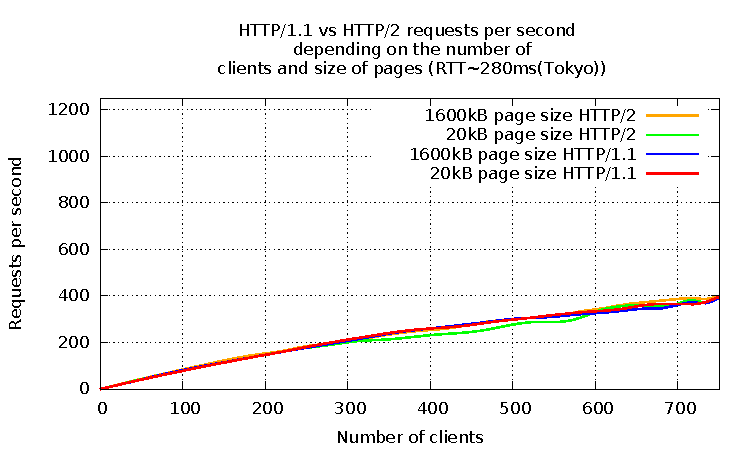
\includegraphics[scale=1,trim=0.0cm .0cm .0cm .0cm,clip]{images/reqps-asia.pdf}
	\caption{Mean Requests per second for Tokyo/Asia}
	\label{fig:reqps-asia}
\end{figure}

\subsubsection{Northcarolina/US}

The next measurements were taken from a client in North America/North Carolina with a measured base average RTT of 150ms and is shown in Figure \ref{fig:latency-na}. 

\begin{figure}[H]
	\centering
	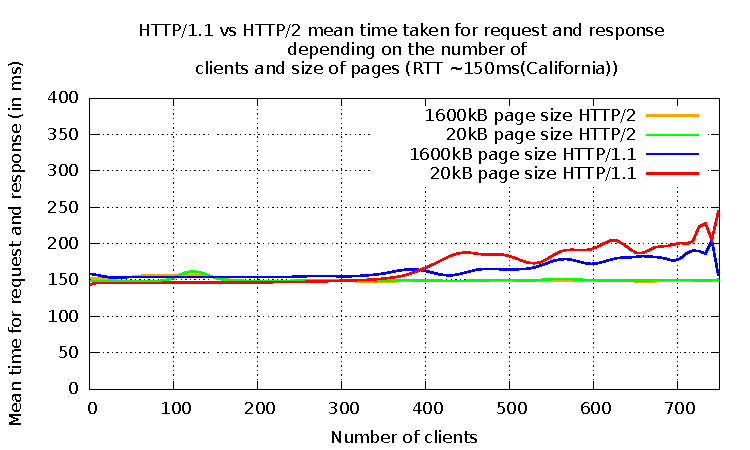
\includegraphics[scale=1,trim=0.0cm .0cm .0cm .0cm,clip]{images/latency-na.pdf}
	\caption{Mean RTT measurements for North Carolina/US}
	\label{fig:latency-na}
\end{figure}

The graph shows for HTTP/2 measurements, that the HTTP RTT is nearly almost equal to the measured base RTT. That means there is almost no jitter measurable and the RTT is constant for HTTP/2 requests regardless if the number of clients is raised or not. Moreover we see a growing HTTP/1.1 RTT starting from approximately 400 concurrent clients upwards. Figure \ref{fig:reqps-na} shows the corresponding request per second rate graph.

\begin{figure}[H]
	\centering
	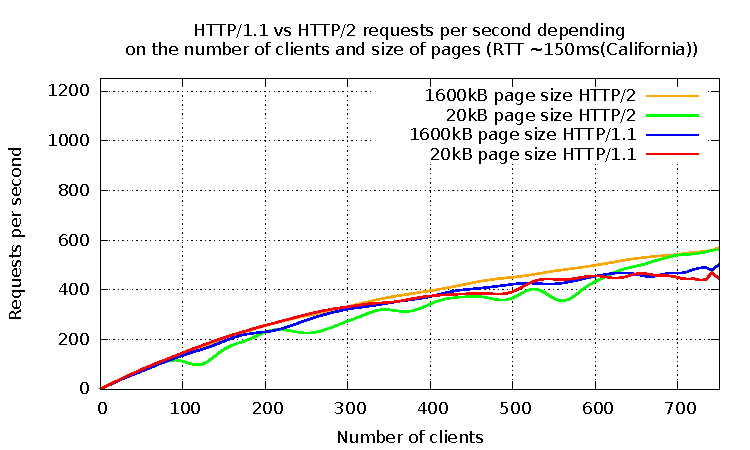
\includegraphics[scale=1,trim=0.0cm .0cm .0cm .0cm,clip]{images/reqps-na.pdf}
	\caption{Mean Requests per second for North Carolina/US}
	\label{fig:reqps-na}
\end{figure}

A slightly better request performance rate for HTTP/2 is the result of that mesurement. 

\subsubsection{Frankfurt am Main/Europe}

Measurements taken from a client in Frankfurt am Main/Germany represent a low latency link with approximately 7ms of base RTT. The graph for the HTTP RTTs is shown in Figure \ref{fig:latency-europe}.

\begin{figure}[H]
	\centering
	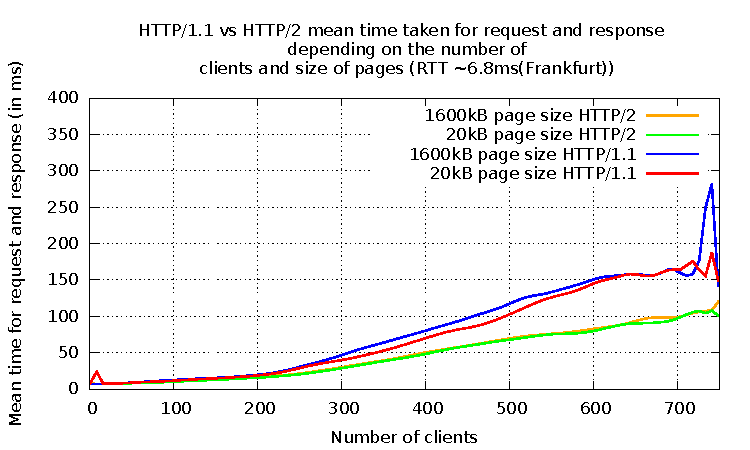
\includegraphics[scale=1,trim=0.0cm .0cm .0cm .0cm,clip]{images/latency-frankfurt.pdf}
	\caption{Mean RTT measurements for Frankfurt am Main/Europe}
	\label{fig:latency-europe}
\end{figure}

Compared to the previous measurements, the RTT graph looks different. Depending on the number of clients the RTT times grow nearly proportional. It is also a clear difference between HTTP/1.1 and HTTP/2 visible. The performed HTTP/2 mesurements show significanltly less growing upto approximately 100ms for 750 clients, whereas the HTTP/1.1 RTT is for all meaurements around 30\% slower ending up in a maximum of around 150ms. The  request rate graph shown in Figure \ref{fig:reqps-frankfurt} shows a different characteristic compared to the previous measurements.

\begin{figure}[H]
	\centering
	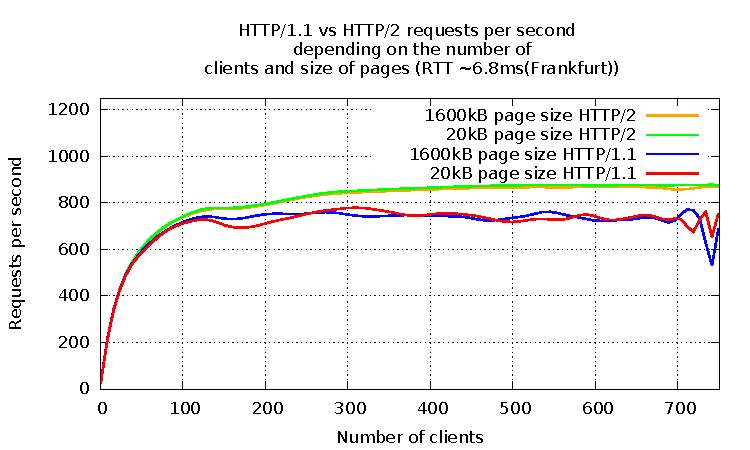
\includegraphics[scale=1,trim=0.0cm .0cm .0cm .0cm,clip]{images/reqps-frankfurt.pdf}
	\caption{Mean Requests per second for Frankfurt/Germany}
	\label{fig:reqps-frankfurt}
\end{figure}

It turns out that the request rate is identical to a asymptotic curve for all measurements. The server simply cannot handle more connection than approximately 800. That is also the reason that after 100 concurrent concurrent clients the request rate remains nearly static. It is again visible that HTTP/2 performs better compared to HTTP/1.1. The fact that the base RTT for that measurement is significantly less than in the previous measurement, leads to much more connections at the same time at the server and different performance graphs.

\subsubsection{Local/Amsterdam}

Finally we performed measurements within the OS3 network (RTT 0.3 ms). We conducted those tests in two different ways. First we did separate measurements for each protocol version and then we conducted parallel tests in order to simulate workloads on the server for HTTP/1.1 and HTTP/2 requests simultanaeous. Figure \ref{fig:latency-local} and Figure \ref{fig:reqps-local} show the graphs for the separate measurements.

\begin{figure}[H]
	\centering
	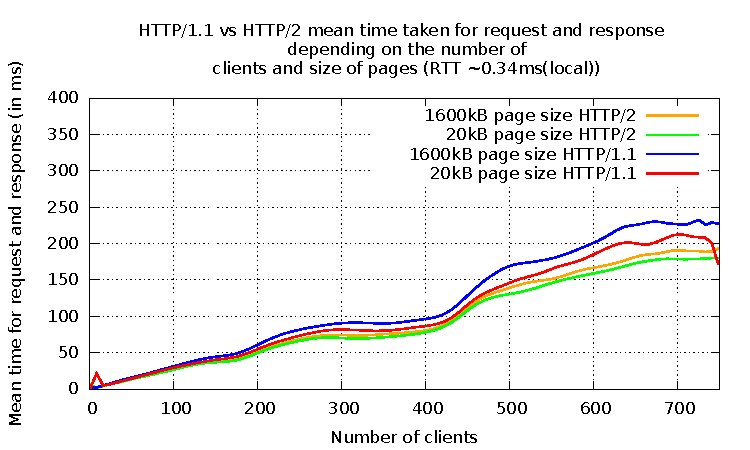
\includegraphics[scale=1,trim=0.0cm .0cm .0cm .0cm,clip]{images/latency-local.pdf}
	\caption{Mean RTT measurements for local/OS3 network}
	\label{fig:latency-local}
\end{figure}

\begin{figure}[H]
	\centering
	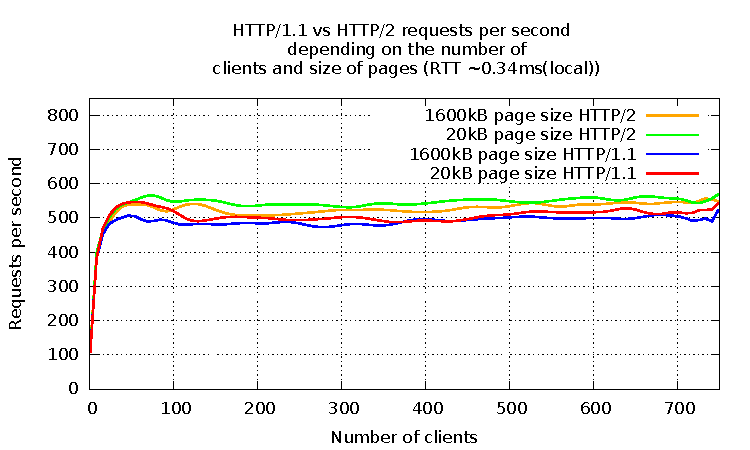
\includegraphics[scale=1,trim=0.0cm .0cm .0cm .0cm,clip]{images/reqps-local.pdf}
	\caption{Mean Requests per second for local/OS3 network}
	\label{fig:reqps-local}
\end{figure}

The graph characteristics is similar to the low latency link in Frankfurt. The difference between both measurements is the number of client needed to reach the server limit in terms or requests per second. The local measurement already reaches that limit at approximately 40 clients. That can be explained by the lower latency within the OS3 network.
\\
\\
As a last measurement we conducted parallel tests for HTTP/1.1 and HTTP/2. The related graphs are shown in Figure \ref{fig:latency-localv1vsv2} and Figure \ref{fig:reqps-localv1vsv2}

\begin{figure}[H]
	\centering
	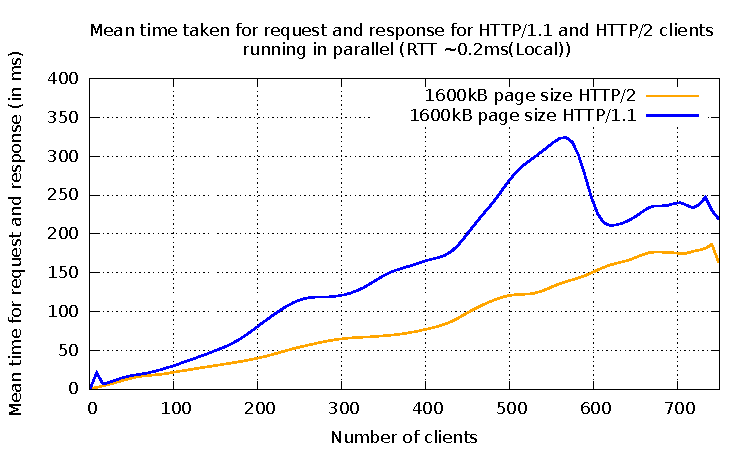
\includegraphics[scale=1,trim=0.0cm .0cm .0cm .0cm,clip]{images/latency-localv1vsv2.pdf}
	\caption{Mean RTT measurements for local parallel/OS3 network}
	\label{fig:latency-localv1vsv2}
\end{figure}

\begin{figure}[H]
	\centering
	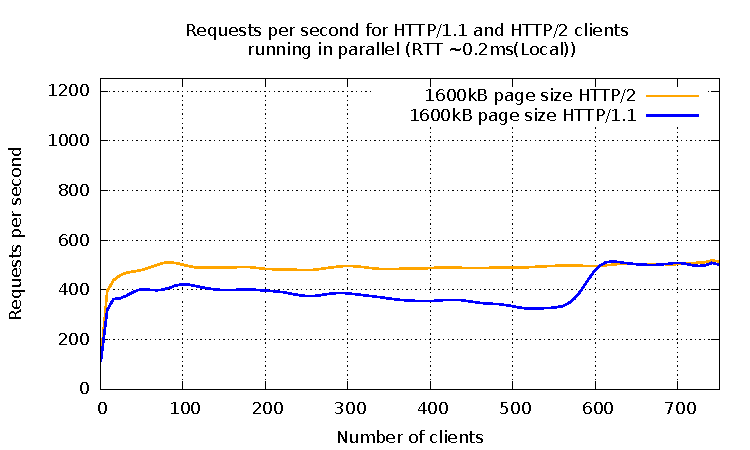
\includegraphics[scale=1,trim=0.0cm .0cm .0cm .0cm,clip]{images/reqps-localv1vsv2.pdf}
	\caption{Mean Requests per second for local parallel/OS3 network}
	\label{fig:reqps-localv1vsv2}
\end{figure}
 
The final result of the local parallel measurements shows again a significant difference between HTTP RTT times of both versions. HTTP/2 is clearly faster than HTTP/1.1. Figure \ref{fig:latency-localv1vsv2} shows a peak RTT for HTTP/1.1 at around 550 clients. At that moment the last HTTP/2 measurement was finished and afterwards the server was only busy with responding to HTTP/1.1 request. That is the reason for the decreasing RTT for HTTP/1.1 and the increasing number of requests per second starting  from that point.

\subsubsection{Mesurement analysis}

We can conclude that for almost all measurements the RTT time for HTTP/2 is significantly faster than for HTTP/1.1. That result is independent of the requested page size and also from the distance between client and server. For high latency links we discovered different characteristics regarding the request rate compared to low latency links (Frankfurt/Local). On low latency links (ca. 10ms) the number of requests per seconds grows much faster, which results in a quick saturation of the server to its maximum number of parallel requests. For high latency links a constant increase of RTT and request rate was measured for an increasing number of clients. In Figure \ref{fig:latency-all} all measured differences between HTTP/1.1 and HTTP/2 for all locations is shown. Lines above zero (y-axis) show a faster RTT for HTTP/2.

\begin{figure}[H]
	\centering
	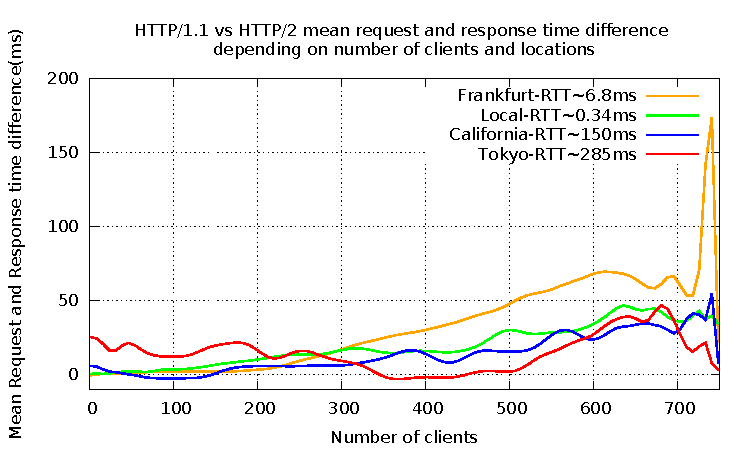
\includegraphics[scale=1,trim=0.0cm .0cm .0cm .0cm,clip]{images/difflatency.pdf}
	\caption{Mean RTT differences HTTP/1.1 - HTTP/2}
	\label{fig:latency-all}
\end{figure}


\subsection{Server Utilization}
\label{subsec:server_util}

During all measuremnts, CPU and network utilization on the server has been monitored and measured. The different results can be categorized into low latency and high latency mesurements. For that reason only the server utilization for the local and North America measurements will be presented. The performance graphs for the server CPU utilization is similar to RTT and request rate graphs and shown in Figure \ref{fig:cpu}   

\begin{figure}[H]
\centering
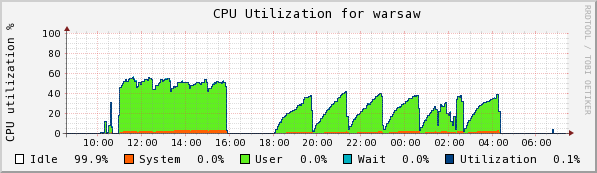
\includegraphics[scale=0.6,trim=0.0cm .0cm .0cm .0cm,clip]{images/cpu.png}
\caption{Server CPU utilization for Local and North America measurements}
\label{fig:cpu}
\end{figure}

The left part of the graph shows the CPU utilization for local measurements (from 11am - 4pm) on the server. A sudden increase up to 60\% which stays until the measurements are finished, is remarkable. That correlates to the graphs for RTT and request rates for local measurements. Starting from 6pm until 4am measurements over a high latency link (North America) were performed. We see a constant growing of the CPU graph until the maximum number of clients of 750 for each test is reached. A nearly identical characteristic shows the bandwidth utilization graph. For the measurements with larger page sizes we see more traffic flowing (Figure \ref{fig:network}).

\begin{figure}[H]
\centering
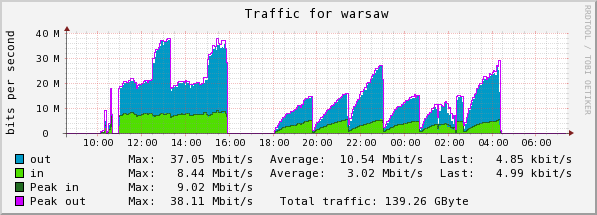
\includegraphics[scale=0.6,trim=0.0cm .0cm .0cm .0cm,clip]{images/network.png}
\caption{Server Bandwidth utilization for Local and North America measurements}
\label{fig:network}
\end{figure}

It is worth to mention that for all HTTP/1.1 measurements a lot of TCP TIME WAIT connections were discovered on the server. TCP TIME WAITS occur when the endpoint (server) blocks a current connection before it can close it due to some missing packets for that particular session. That happens because the server has much more TCP connections to manage for HTTP/1.1. The graph representing the TCP socket states on the server is shown in Figure \ref{fig:sockets}

\begin{figure}[H]
\centering
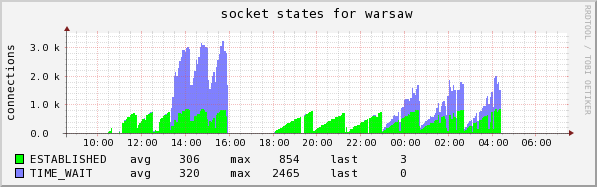
\includegraphics[scale=0.6,trim=0.0cm .0cm .0cm .0cm,clip]{images/sockets.png}
\caption{Server sockets for Local and North America measurements}
\label{fig:sockets}
\end{figure}
\newpage
\section{Conclusions}
\label{conclusion}
\newpage
\section{Future Work}
\label{furtherwork}
\newpage
\begin{thebibliography}
\\
\bibitem{RFC2616}
RFC2616, Fielding, R., Gettys, J., Mogul, J., Frystyk, H., Masinter, L., Leach, P., and T. Berners-Lee, "Hypertext Transfer Protocol -- HTTP/1.1", RFC 2616, June 1999, Available at: http://www.rfc-editor.org/info/rfc2616 .[Accessed 26 Mar. 2015].
\bibitem{RFC723x}
RFC7230 Fielding, R., Ed., and J. Reschke, Ed., "Hypertext Transfer Protocol (HTTP/1.1): Message Syntax and Routing", RFC 7230, June 2014, Available at:http://www.rfc-editor.org/info/rfc7230  [Accessed 26 Mar. 2015]. \\
RFC7231 Fielding, R., Ed., and J. Reschke, Ed., "Hypertext Transfer Protocol (HTTP/1.1): Semantics and Content", RFC 7231, June 2014, Available at: http://www.rfc-editor.org/info/rfc7231 [Accessed 26 Mar. 2015]. \\
RFC7232 Fielding, R., Ed., and J. Reschke, Ed., "Hypertext Transfer Protocol (HTTP/1.1): Conditional Requests", RFC 7232, June 2014, Available at: http://www.rfc-editor.org/info/rfc7232 [Accessed 26 Mar. 2015]. \\ 
RFC7233 Fielding, R., Ed., Lafon, Y., Ed., and J. Reschke, Ed., "Hypertext Transfer Protocol (HTTP/1.1): Range Requests", RFC 7233, June 2014, Available at: http://www.rfc-editor.org/info/rfc7233 [Accessed 26 Mar. 2015]. \\
RFC7234 Fielding, R., Ed., Nottingham, M., Ed., and J. Reschke, Ed., "Hypertext Transfer Protocol (HTTP/1.1): Caching", RFC 7234, June 2014, Available at: http://www.rfc-editor.org/info/rfc7234 [Accessed 26 Mar. 2015]. \\
RFC7235 Fielding, R., Ed., and J. Reschke, Ed., "Hypertext Transfer Protocol (HTTP/1.1): Authentication", RFC 7235, June 2014, Available at: http://www.rfc-editor.org/info/rfc7235 [Accessed 26 Mar. 2015].
\bibitem{http2}
Hypertext Transfer Protocol version 2 (draft-ietf-httpbis-http2-17) (2015). M. Belshe, Twist R. Peon [online] IETF, Available at:
https://datatracker.ietf.org/doc/draft-ietf-httpbis-http2/?include\_text=1 [Accessed 26 Mar. 2015].
 \bibitem{hpack}
HPACK - Header Compression for HTTP/2 draft-ietf-httpbis-header-compression-07 (2015). R. Peon,  H. Ruellan [online] IETF, Available at: http://tools.ietf.org/html/draft-ietf-httpbis-header-compression-07 [Accessed 26 Mar. 2015].
\bibitem{google2x}
A 2x Faster Web. (2009). [online] Chromium Blog. Available at: http://blog.chromium.org/2009/11/2x-faster-web.html [Accessed 20 Feb. 2015].
\bibitem{servy}
Servy, H. (2015). Evaluating the Performance of SPDY-enabled Web Servers. [online] Neotys.com. Available at: http://www.neotys.com/blog/performance-of-spdy-enabled-web-servers/ [Accessed 20 Feb. 2015].
\bibitem{podiatry}
Podiatry, G. (2015). Guy's Pod » Blog Archive » Not as SPDY as You Thought. [online] Guypo.com. Available at: http://www.guypo.com/not-as-spdy-as-you-thought/ [Accessed 20 Feb. 2015].
\bibitem{wang}
Wang et al. (2014). How Speedy is SPDY?, 11th USENIX Symposium on Networked Systems Design and Implementation (NSDI ’14). [online] usenix.org. Available at:
https://www.usenix.org/system/files/conference/nsdi14/nsdi14-paper-wang\_xiao\_sophia.pdf [Accessed 20 Feb. 2015].
\bibitem{amazon} Amazon Elastic Compute Cloud (Amazon EC2) (2015). Available at: http://aws.amazon.com/ec2/ [Accessed 20 Feb. 2015].
\bibitem{mozilla} Firefox Beta Notes (2015). Available at: https://www.mozilla.org/en-US/firefox/36.0beta/releasenotes/ [Accessed 20 Feb. 2015].
\bibitem{http2-imp}  HTTP/2 client/server implemenations (2015). Available at: https://github.com/http2/http2-spec/wiki/Implementations [Accessed 20 Feb. 2015].
\bibitem{h2c-14} Hypertext Transfer Protocol version 2 draft-ietf-httpbis-http2-14 (2014). Available at: https://tools.ietf.org/html/draft-ietf-httpbis-http2-14 [Accessed 4. March 2015]
\bibitem{nghttp} HTTP/2 experimental server (2015). Available at: https://nghttp2.org/documentation/nghttpd.1.html [Accessed 4. March 2015]
\bibitem{apache2} The Apache HTTP Server Project (2015). Available at: http://httpd.apache.org/ [Accessed 4. March 2015]
\bibitem{h2load} Benchmarking tool for HTTP/2 and SPDY server (2015). Available at: https://nghttp2.org/documentation/h2load.1.html [Accessed 4. March 2015]
\bibitem{ab} Apache HTTP server benchmarking tool (2015). Available at http://httpd.apache.org/docs/2.2/programs/ab.html [Accessed 4. March 2015]
\bibitem{httparchive} Httparchive.org, (2015). HTTP Archive - Trends. [online] Available at: http://httparchive.org/trends.php [Accessed 11 Mar. 2015].
\bibitem{amazon-ts} amazon.com, (2015). Amazon - T2 Instances. [online] Available at: http://docs.aws.amazon.com/AWSEC2/latest/UserGuide/t2-instances.html [Accessed 11 Mar. 2015].
\bibitem{nghttpx} nghttp2.org, nghttpx HTTP/1.1 HTTP/2 reverse proxy. [online] Available at: https://nghttp2.org/documentation/nghttpx.1.html [Accessed 28 Mar. 2015].
\bibitem{apache} Apache Web Server (2015). Available at: http://httpd.apache.org/  [Accessed 11 Mar. 2015].
\end{thebibliography}



\end{document}
